
  % ------------------------------------------------------------------------
  % abnTeX2: Modelo de Trabalho Academico (tese de doutorado, dissertacao de
  % mestrado e trabalhos monograficos em geral) em conformidade com
  % ABNT NBR 14724:2011: Informacao e documentacao - Trabalhos academicos -
  % Apresentacao
  % ------------------------------------------------------------------------
  % ------------------------------------------------------------------------

  \documentclass[
    % -- opções da classe memoir --
    12pt,       % tamanho da fonte
    openright,      % capítulos começam em pág ímpar (insere página vazia caso preciso)
    twoside,      % para impressão em verso e anverso. Oposto a oneside
    a4paper,      % tamanho do papel.
    % -- opções da classe abntex2 --
    %chapter=TITLE,   % títulos de capítulos convertidos em letras maiúsculas
    %section=TITLE,   % títulos de seções convertidos em letras maiúsculas
    %subsection=TITLE,  % títulos de subseções convertidos em letras maiúsculas
    %subsubsection=TITLE,% títulos de subsubseções convertidos em letras maiúsculas
    % -- opções do pacote babel --
    english,      % idioma adicional para hifenização
    french,       % idioma adicional para hifenização
    spanish,      % idioma adicional para hifenização
    brazil,       % o último idioma é o principal do documento
    ]{abntex2}


  % ---
  % PACOTES
  % ---

  % ---
  % Pacotes fundamentais
  % ---
  \usepackage{cmap}       % Mapear caracteres especiais no PDF
  \usepackage{lmodern}      % Usa a fonte Latin Modern
  \usepackage[T1]{fontenc}    % Selecao de codigos de fonte.
  \usepackage[utf8]{inputenc}   % Codificacao do documento (conversão automática dos acentos)
  \usepackage{lastpage}     % Usado pela Ficha catalográfica
  \usepackage{indentfirst}    % Indenta o primeiro parágrafo de cada seção.
  \usepackage{color}        % Controle das cores
  \usepackage{graphicx}     % Inclusão de gráficos
  \usepackage{listings}     % Inclusão de código
  \usepackage[final]{pdfpages}
  \usepackage{algorithm}
  \usepackage{algorithmic}
  \usepackage{color}
  \usepackage[section]{placeins}
  \usepackage{csquotes}
  \usepackage{longtable}

  % ---
  % Pacotes de citações
  % ---
  \usepackage[brazilian,hyperpageref]{backref}   % Paginas com as citações na bibl
  \usepackage[alf]{abntex2cite} % Citações padrão ABNT

  % ---
  % CONFIGURAÇÕES DE PACOTES
  % ---

  % ---
  % Configurações do pacote backref
  % Usado sem a opção hyperpageref de backref
  \renewcommand{\backrefpagesname}{Citado na(s) página(s):~}
  % Texto padrão antes do número das páginas
  \renewcommand{\backref}{}
  % Define os textos da citação
  \renewcommand*{\backrefalt}[4]{
    \ifcase #1 %
      Nenhuma citação no texto.%
    \or
      Citado na página #2.%
    \else
      Citado #1 vezes nas páginas #2.%
    \fi}%
    
\renewcommand{\lstlistingname}{Código}
  % ---

  % ---
  % Informações de dados para CAPA e FOLHA DE ROSTO
  % ---
  \titulo{Um estudo de caso de gestão de riscos aplicada a métodos ágeis}
  \autor{Fernanda Narloch Rizzo Hahn}
  \local{Florianópolis}
  \data{2021}
  \orientador{Jean Carlo Rossa Hauck}
  \coorientador{}
  \instituicao{%
    Universidade Federal de Santa Catarina
    \par
    Centro Tecnológico - CTC
    \par
    Departamento de Informática e Estatística
    \par
    Ciências da Computação}
  \tipotrabalho{Dissertação (Bacharelado)}

  \preambulo{Trabalho de Conclusão de Curso submetido ao Curso de
  Ciências da Computação para a obtenção do Grau de Bacharel em
  Ciências da Computação.}
  % ---

  % ---
  % Configurações de aparência do PDF final

  % alterando o aspecto da cor azul
  \definecolor{blue}{RGB}{41,5,195}

  % informações do PDF
  \makeatletter
  \hypersetup{
        %pagebackref=true,
      pdftitle={\@title},
      pdfauthor={\@author},
        pdfsubject={\imprimirpreambulo},
        pdfcreator={LaTeX with abnTeX2},
      pdfkeywords={abnt}{latex}{abntex}{abntex2}{trabalho acadêmico},
      colorlinks=true,          % false: boxed links; true: colored links
        linkcolor=black,           % color of internal links
        citecolor=black,           % color of links to bibliography
        filecolor=magenta,          % color of file links
      urlcolor=blue,
      bookmarksdepth=4
  }
  \makeatother
  % ---
  % ---
  % Espaçamentos entre linhas e parágrafos
  % ---

  % O tamanho do parágrafo é dado por:
  \setlength{\parindent}{1.3cm}

  % Controle do espaçamento entre um parágrafo e outro:
  \setlength{\parskip}{0.2cm}  % tente também \onelineskip

  % ---
  % compila o indice
  % ---
  \makeindex
  % ---

  % ----
  % Início do documento
  % ----
  \begin{document}
  % Retira espaço extra obsoleto entre as frases.
  \frenchspacing

  % ----------------------------------------------------------
  % ELEMENTOS PRÉ-TEXTUAIS
  % ----------------------------------------------------------
  % \pretextual

  % ---
  % Capa
  % ---
  \imprimircapa
  % ---

  % ---
  % Folha de rosto
  % (o * indica que haverá a ficha bibliográfica)
  % ---
  \imprimirfolhaderosto*
  % ---
  
  % ---
  % Inserir folha de aprovação
  % ---

  % Isto é um exemplo de Folha de aprovação, elemento obrigatório da NBR
  % 14724/2011 (seção 4.2.1.3). Você pode utilizar este modelo até a aprovação
  % do trabalho. Após isso, substitua todo o conteúdo deste arquivo por uma
  % imagem da página assinada pela banca com o comando abaixo:
  %
  % \includepdf{folhadeaprovacao_final.pdf}
  %
  \begin{folhadeaprovacao}

    \begin{center}
      {\ABNTEXchapterfont\large\imprimirautor}

      \vspace*{\fill}
      {\ABNTEXchapterfont\large\bfseries\imprimirtitulo}
      \vspace*{\fill}


     Este Trabalho de Conclusão de Curso foi julgado aprovado para a
     obtenção do Título de Bacharel em Ciências da Computação, e
     aprovado em sua forma final pelo Curso de Ciências da Computação
     da Universidade Federal de Santa Catarina.
     \end{center}

     \assinatura{Dr. Prof. \imprimirorientador \\ Orientador}
     \assinatura{Dr. Prof.  \\ Avaliador}
     \assinatura{Dr. Prof.  \\ Avaliador}
     %\assinatura{\textbf{Professor} \\ Convidado 3}
     %\assinatura{\textbf{Professor} \\ Convidado 4}

     \begin{center}
      \vspace*{0.5cm}
      {\large\imprimirlocal}
      \par
      {\large\imprimirdata}
      \vspace*{1cm}
    \end{center}

  \end{folhadeaprovacao}
  % ---

  % ---
  % Agradecimentos
  % ---
  \begin{agradecimentos}
  \end{agradecimentos}
  % ---

  % ---
  % Epígrafe
  % ---
  \begin{epigrafe}
      \vspace*{\fill}
    \begin{flushright}
      \textit{“As long as you are learning, you are not failing.” – Bob Ross}
    \end{flushright}
  \end{epigrafe}
  % ---

  % ---
  % RESUMOS
  % ---

  % resumo em português
  \begin{resumo}
    A popularização dos métodos ágeis no desenvolvimento de \textit{software} trouxe maior velocidade e flexibilidade aos projetos que anteriormente eram desenvolvidos com base em modelos prescritivos. Contudo, os métodos ágeis não são capazes de prevenir por si características típicas de projetos de \textit{software} como a imprevisibilidade e instabilidade. Pois, esses modelos de gerência de projeto não contam com técnicas formais de gestão de riscos para lidar com as incertezas existentes durante o desenvolvimento. Essa lacuna pode provocar o fracasso de um ou mais objetivos do projeto ao preterir a identificação de riscos potencias e consequentemente não dispor de um plano de contingência. Dessa forma, foi criado o “Guia para gestão ágil de riscos em projetos de software” no contexto do Grupo de Qualidade de Software (GQS/INE/CTC/UFSC) com o intuito de apresentar diretrizes que visam auxiliar a prática da gestão explícita de riscos no ambiente de desenvolvimento ágil de software. Assim, o presente trabalho se trata de um estudo de caso que pretende aplicar e avaliar técnicas de gestão de riscos do Guia em equipes ágeis do Laboratório Bridge da Universidade Federal de Santa Catarina. Para isso, inicialmente serão revisados conceitos fundamentais referentes ao tema e também será realizada a análise do estado da arte na área. Com base nos conhecimentos adquiridos e no “Guia para gestão ágil de riscos em projetos de software” será desenvolvido um diagnóstico inicial do contexto do Laboratório Bridge e, a partir dele, serão propostas as técnicas a serem aplicadas durante o estudo de caso. Após a implantação das técnicas, será realizada a avaliação dos resultados obtidos.
   \vspace{\onelineskip}

   \noindent
   \textbf{Palavras-chaves}: Gestão de Riscos, Gestão de Projetos, Métodos Ágeis, Desenvolvimento de Software
  \end{resumo}

  % resumo em inglês
  \begin{resumo}[Abstract]
   \begin{otherlanguage*}{english}
TODO
     \vspace{\onelineskip}

     \noindent
     \textbf{Key-words}: TODO
   \end{otherlanguage*}
  \end{resumo}
  % ---

  % ---
  % inserir lista de ilustrações
  % ---
  \pdfbookmark[0]{\listfigurename}{lof}
  \listoffigures*
  \cleardoublepage
  % ---

  % ---
  % inserir lista de tabelas
  % ---
  \pdfbookmark[0]{\listtablename}{lot}
  \listoftables*
  \cleardoublepage
  % ---

  % ---
  % inserir lista de abreviaturas e siglas
  % ---
  \begin{siglas}
    \item[IT] Item
 \end{siglas}
  % ---

  % ---
  % inserir o sumario
  % ---
  \pdfbookmark[0]{\contentsname}{toc}
  \tableofcontents*
  \cleardoublepage
  % ---



  % ----------------------------------------------------------
  % ELEMENTOS TEXTUAIS
  % ----------------------------------------------------------
  \textual


  % ----------------------------------------------------------
  % PARTE - preparação da pesquisa
  % ----------------------------------------------------------
\chapter{Introdução e objetivos}
\label{sec:Introducao}
\section{Introdução}

Na busca pela obtenção de vantagens competitivas, surgiu a necessidade de substituir modelos prescritivos por adaptativos no processo de desenvolvimento de software. De forma geral, os modelos adaptativos preveem práticas mais flexíveis e com maior enfoque na agilidade, preservando ainda a qualidade do produto \cite{Rech:2013}. Mesmo com essa crescente popularidade das métodos ágeis, o relatório CHAOS Report 2015 conduzido pelo \citeonline{StandishGroup:2014}  apresentou que apenas 39\% dos projetos de software que utilizaram métodos ágeis foram bem-sucedidos. Apesar desse cenário e do fato de riscos serem uma constante durante o desenvolvimento de software \cite{Cunha:2013}, os método ágeis não contam com uma formalização de técnicas para a gerência de riscos \cite{Tomanek:2015}.

No contexto de gerenciamento de projetos, riscos são uma condição de incerteza que pode ocasionar efeitos positivos ou negativos no projeto \cite{PMBOK:2017}. Segundo o PMBOK, o gerenciamento dos riscos de um projeto tipicamente inclui os processos Planejar o Gerenciamento dos Riscos, Identificar os Riscos, Realizar a Análise Qualitativa dos Riscos, Realizar a Análise Quantitativa dos Riscos, Planejar as Respostas aos Riscos, Implementar Respostas a Riscos e Monitorar Riscos. 

O primeiro se trata do processo para definir qual será a abordagem de gerência de riscos utilizada no projeto. Já Identificar Riscos é o processo de identificar possíveis fontes de risco bem como riscos individuais e documentá-los. Na Análise Qualitativa dos Riscos é realizada a avaliação da probabilidade de ocorrência e impacto de cada risco, a partir disso é possível classificar os riscos quanto a prioridade. A Análise Quantitativa dos Riscos denota o processo de estimar numericamente o efeito combinado dos riscos nos objetivos do projeto. O Planejamento de Respostas aos Riscos é o processo de identificar estratégias de resposta para cada risco identificado, que serão efetuadas no processo Implementar Respostas. Por fim, Monitorar os riscos é o processo de monitorar tanto a implementação das estratégias acordadas, quanto acompanhar os riscos já identificados e identificar novos riscos \cite{PMBOK:2017}.

As técnicas de gerenciamento de riscos possibilitam a redução do impacto negativo e a potencialização do impacto positivo dos riscos \cite{Milare:2019}. Uma pesquisa realizada em 2015, através de entrevistas com gerentes de projeto experientes que utilizam métodos ágeis, concluiu que a gestão proativa de riscos aplicada a modelos adaptativos influencia positivamente o resultado do projeto. E, também pontuou que, apesar dos métodos ágeis já minimizarem os cenários negativos através da aplicação de iterações curtas, a gestão de riscos atua como um complemento, sendo assim, capaz de aperfeiçoar o projeto em questões relacionadas a fatores críticos de sucesso, custo, tempo e qualidade \cite{Gold:2015}.

Diversas iniciativas têm surgido no intuito de auxiliar as organizações de software que utilizam métodos ágeis a adotar técnicas explícitas de gestão de riscos. Um desses trabalhos é o “Guia para gestão ágil de riscos em projetos de software” desenvolvido no contexto do Grupo de Qualidade de Software (GQS/INE/CTC/UFSC). O conteúdo do guia foi fundamentado através da análise da literatura, da identificação do estado da arte na área de gestão ágil de riscos e das experiências empíricas dos autores. E, dispõe de diretrizes que visam auxiliar a prática da gestão explícita de riscos no ambiente de desenvolvimento ágil de software \cite{Vieira:2020}. Contudo, o guia ainda não foi aplicado em um contexto real.

A partir do panorama apresentado, este trabalho objetiva realizar um estudo de caso para avaliar o impacto da introdução de práticas explícitas de gerência de riscos no processo de desenvolvimento ágil de software. A aplicação do estudo de caso busca selecionar empiricamente quais técnicas utilizadas na gestão de riscos se enquadram melhor no contexto do Laboratório Bridge da Universidade Federal de Santa Catarina, por meio da adoção de técnicas propostas no “Guia para gestão ágil de riscos” \cite{Vieira:2020} em equipes da organização durante o segundo semestre letivo de 2021. O Laboratório Bridge é um laboratório integrado ao Centro Tecnológico (CTC) e de Ciências da Saúde (CCS) da Universidade Federal de Santa Catarina (UFSC) criado em 2013. Atua na pesquisa e desenvolvimento de soluções tecnológicas para o Ministério da Saúde, como por exemplo softwares para a estratégia e-SUS APS, Sistema de Monitoramento de Obras (SISMOB) e Registro Nacional de Implantes (RNI). Conta com 123 colaboradores divididos em 6 áreas/projetos, sendo o maior projeto o e-SUS APS com 64 colaboradores distribuídos em 8 equipes ágeis.

Para o desenvolvimento do estudo de caso, primeiramente será realizado um estudo inicial sobre o processo do laboratório bem como a organização desse. Após, utilizando como base a literatura, serão selecionadas técnicas do “Guia para gestão ágil de riscos” \cite{Vieira:2020} que melhor se enquadram com as características do Laboratório Bridge. A cada sprint, uma técnica escolhida será aplicada a uma equipe ágil participante. Ao final da iteração, será avaliado se a técnica trouxe algum benefício para o desempenho da equipe. Dessa forma, será possível definir quais técnicas são mais adequadas ao ambiente ágil do laboratório, bem como quais melhorias essas trouxeram ao processo da organização.

\section{Objetivo geral}

O presente trabalho tem como objetivo geral aplicar e avaliar as técnicas de gestão de riscos presentes no “Guia para gestão ágil de riscos” \cite{Vieira:2020} em um contexto real de desenvolvimento de software, por meio de um estudo de caso aplicado a equipes ágeis do Laboratório Bridge da Universidade Federal de Santa Catarina.

\section{Objetivos específicos}
\begin{enumerate}
     \item Realizar uma análise da literatura quanto ao estado da arte da gestão de risco aplicada a métodos ágeis
    \item Realizar um diagnóstico inicial dos processos da unidade organizacional;
    \item Propor técnicas de gestão de risco do “Guia para gestão ágil de riscos” \cite{Vieira:2020} a serem serem aplicadas na unidade organizacional durante estudo de caso;
    \item Avaliar os impactos no processo a partir da aplicação das técnicas e quais técnicas melhor se encaixaram no perfil da unidade organizacional;
\end{enumerate}

\section{Metodologia de pesquisa}

Este trabalho pretende aplicar técnicas de gestão de riscos presentes no “Guia para gestão ágil de riscos”  \cite{Vieira:2020} em uma unidade organizacional e observar, analisar e discutir os impactos dessa aplicação no contexto das equipes ágeis de desenvolvimento de \textit{software}.

Segundo \citeonline{Yin:2001}, “Um estudo de caso é uma investigação empírica que investiga um fenômeno contemporâneo dentro de seu contexto da vida real, especialmente quando os limites entre o fenômeno e o contexto não estão claramente
definidos.”. 

Conforme este conceito de classificação metodológica, o presente trabalho será um estudo de caso, com objetivo exploratório, aplicado dentro de um ambiente real de um laboratório de desenvolvimento de \textit{software}. Para alcançar os objetivos definidos no trabalho, a metodologia adotada foi definida através das três etapas demonstradas a seguir: 

\begin{itemize}[label={}]
  \item \textbf{Etapa 1. Fundamentação Teórica - } Nesta primeira etapa serão revisados conceitos fundamentais da literatura relacionados a gerência de projetos, métodos ágeis e gestão de riscos. As seguintes atividades compõe a etapa:
    \begin{itemize}[label={}]
        \item \textbf{Atividade 1.1 - } Fundamentar principais conceitos sobre gerência de projeto.
        \item \textbf{Atividade 1.2 - } Fundamentar principais conceitos sobre métodos ágeis.
        \item \textbf{Atividade 1.3 - } Fundamentar principais conceitos sobre gestão de riscos. 
    \end{itemize}
  
  
  \item \textbf{Etapa 2. Análise do estado da arte - } A análise do estado da arte possui caráter bibliográfico e objetiva mapear e discutir produções acadêmicas em um campo de conhecimento \cite{Ferreira:2002}. Assim, nesta etapa será realizada uma revisão sistemática da literatura a partir de critérios de pesquisa para o levantamento de estudos correlacionados com o tema deste trabalho. Esta etapa é composta pelas seguintes atividades:
    \begin{itemize}[label={}]
        \item \textbf{Atividade 2.1 - } Especificação do problema.
        \item \textbf{Atividade 2.2 - } Definição das perguntas de pesquisa.
        \item \textbf{Atividade 2.3 - } Identificação dos critérios de pesquisa. 
        \item \textbf{Atividade 2.4 - } Seleção de estudos relacionados a este trabalho. 
        \item \textbf{Atividade 2.5 - } Extração e análise de dados.
    \end{itemize}
  

  \item \textbf{Etapa 3. Definição, aplicação e análise do estudo de caso - } Na terceira e última etapa será planejado e realizado o estudo de caso conforme as atividades abaixo:
      \begin{itemize}[label={}]
        \item \textbf{Atividade 3.1 - } Diagnóstico do contexto da unidade organizacional.
        \item \textbf{Atividade 3.2 - } Definição do estudo.
        \item \textbf{Atividade 3.3 - } Planejamento do estudo. 
        \item \textbf{Atividade 3.4 - } Aplicação do estudo. 
        \item \textbf{Atividade 3.5 - } Análise dos resultados. 
    \end{itemize}

\end{itemize}

\chapter{Fundamentação teórica}
\label{sec:Fundamentacao}

Neste capítulo serão apresentados conceitos relevantes relacionados a gerência de projetos, gestão de riscos e métodos ágeis que serão abordados no decorrer deste trabalho.

\section{Gerência de projetos}

Segundo o PMBOK \cite{PMBOK:2017}: "Projeto é um esforço temporário empreendido para criar um produto, serviço ou resultado único.". Os projetos são de natureza temporária, assim, devem possuir data de início e término definidas. Eles se dão por concluídos quando os objetivos são alcançados ou quando o projeto falha por algum fator como, por exemplo, recursos esgotados, mudança de estratégia ou motivos legais. Um projeto que obtenha sucesso no cumprimento dos objetivos gerará, então, um produto, serviço ou resultado único. 

A área de gerência de projetos objetiva que estes empreendimentos temporários sejam executados de forma eficaz e eficiente. Para que, dessa maneira, as organizações sejam bem sucedidas no cumprimento dos requisitos dos projetos. Este suporte é realizado através da aplicação de conhecimentos, habilidades, ferramentas e técnicas às atividades do projeto \cite{PMBOK:2017}. 

A gerência de projetos identifica componentes-chave dos projetos que devem ser bem gerenciados para que o empreendimento obtenha êxito. Tais componentes estão descritos na Tabela \ref{tab:KeyComponents}.

\begin{longtable}{p{5cm}p{10cm}}
    \caption{Descrição dos componentes-chaves de um projeto}
    \label{tab:KeyComponents}
    \centering
              \cr \textbf{Componentes-Chave} & \textbf{Descrição} 
              \\ \hline \addlinespace[0.3cm]
              \textbf{Ciclo de vida do projeto} &
              A série de fases pelas quais um projeto passa, do início ao término.
              \\\addlinespace[0.3cm] \hline \addlinespace[0.3cm]
              
              \textbf{Fase do projeto} &
              Um conjunto de atividades do projeto relacionadas de maneira lógica que culmina na conclusão de uma ou mais entregas
              \\\addlinespace[0.3cm] \hline \addlinespace[0.3cm]
              
                
              \textbf{Revisão de fase} &
              Uma análise no final de uma fase em que uma decisão é tomada em relação a passar para a fase seguinte, continuar com modificações ou finalizar um programa ou projeto.
              \\\addlinespace[0.3cm] \hline \addlinespace[0.3cm]
              
              \textbf{Processos de gerenciamento de projetos} &
              Uma série de atividades sistemáticas direcionadas para alcançar um resultado final de tal forma que se aja em relação a uma ou mais entradas a fim de criar uma ou mais saídas.
              \\\addlinespace[0.3cm] \hline \addlinespace[0.3cm]
              
              \textbf{Grupo de processos de gerenciamento de projetos} &
              Um agrupamento lógico de entradas, ferramentas, técnicas e saídas de gerenciamento de projetos. Os grupos de processos de gerenciamento de projetos incluem iniciar, planejar, executar, monitorar, controlar e encerrar. Os grupos de processos de gerenciamento de projetos não são fases do projeto.
              \\\addlinespace[0.3cm] \hline \addlinespace[0.3cm]
              
              \textbf{Área de conhecimento em gerenciamento de projetos} &
              Uma área identificada de gerenciamento de projetos definida por seus requisitos de conhecimentos e descrita em termos dos processos que a compõem: suas práticas, entradas, saídas, ferramentas e técnicas.
              \\\addlinespace[0.3cm] \hline \addlinespace[0.5cm]
                 
              \caption*{\textbf{Fonte:} Adaptado de PMBOK \cite{PMBOK:2017}}
\end{longtable}



\section{Gestão de riscos}

Em 1983, a Royal Society britânica publicou um relatório denominado \textit{"Risk assessment: a Study Group Report"}, que definiu risco como: A probabilidade de que um determinado evento adverso ocorra durante um período de tempo definido ou resulte de determinado desafio. Como na probabilidade no sentido da teoria estatística, o risco obedece a todas as leis formais das probabilidades combinatórias \cite{ADAMS:1995}. 

Já o PMBOK \cite{PMBOK:2017} inclui neste conceito a possibilidade de que riscos tenham também um efeito positivo no projeto. No guia são definidos dois tipos de risco: o risco individual do projeto e o risco geral do projeto. Para o PMBOK, o primeiro "é um evento ou condição incerta que, se ocorrer, provocará um efeito positivo ou
negativo em um ou mais objetivos do projeto.". E o risco geral do projeto " é o efeito da incerteza do projeto no seu todo, decorrente de todas as fontes de incerteza, incluindo riscos individuais, representando a exposição das partes interessadas às implicações de variações no resultado do projeto, sejam positivas ou negativas."

Para \citeonline{WAZLAWICK:2013}, os riscos estão presentes em todos os projetos de desenvolvimento de software e, caso não se esteja atento a eles, os riscos podem prejudicar ou até mesmo inviabilizar um projeto. Ademais, de uma maneira genérica, é possível afirmar que negligenciar o planejamento em relação aos riscos é uma das maiores razões para o insucesso de um projeto de software.

Assim, a motivação para a gestão de risco se dá pelo fato de que riscos negativos (ameaças) não administrados podem gerar efeitos negativos no projeto, ou então, podem ser perdidos riscos positivos (oportunidades) não identificados. Assim, o objetivo da gestão de risco é potencializar as oportunidades e minimizar as ameaças \cite{PMBOK:2017}.

\subsection{Planejar o Gerenciamento dos Riscos}
\subsection{Identificar os Riscos}
\subsection{Realizar a Análise Qualitativa dos Riscos}
\subsection{Realizar a Análise Quantitativa dos Riscos}
\subsection{Implementar Respostas aos Riscos}
\subsection{Monitorar Riscos}

\section{Métodos ágeis}

Na década de 1980 e início de 1990, acreditava-se que o processo de desenvolvimento de software deveria ser minuciosamente planejado e monitorado. Tal noção advém principalmente dos primórdios da engenharia de software, que surgiu dentro de um contexto de softwares robustos e duradouros como sistemas aeroespaciais e softwares de governo. 

Porém, essa abordagem tradicional de desenvolvivemento, quando aplicada a softwares corporativos de portes pequenos e médios, acaba prejudicando o andamento do projeto. Isso ocorre porque gasta-se mais tempo no planejamento e análise do projeto do que de fato no desenvolvimento. Além disso, tais sistemas costumam possuir requisitos mutáveis, o que envolve modificações no código e a adaptação das especificações. 

Neste cenário de insatisfação, surgiram os métodos ágeis que possuem como principal característica a utilização de uma abordagem incremental tanto para a especificação do sistema quanto para o desenvolvimento e entrega. Assim, os métodos ágeis permitem que os softwares sejam rapidamente entregues e facilmente adaptáveis a novos requisitos \cite{SOMMERVILLE:2011}.

A filosofia dos métodos ágeis foi descrita em 2001 por um grupo de 17 desevolvedores de software através do Manifesto Ágil \cite{AGILEMANIFEST:2001}. Tal manifesto possui quatro valores:

\begin{itemize}
        \item Indivíduos e interações mais que processos e ferramentas;
        \item Software em funcionamento mais que documentação abrangente;
        \item Colaboração com o cliente mais que negociação de contratos;
        \item Responder a mudanças mais que seguir um plano;
\end{itemize}

E, embora processos e ferramentas, documentação abrangente, negociação de contratos e seguir um plano sejam importantes, o manifesto valoriza mais os pontos à esquerda: Indivíduos e interações, software em funcionamento, colaboração com o cliente e resposta à mudanças. No livro Engenharia de Software, \citeonline{WAZLAWICK:2013} salienta que a cultura ágil não abandona planejamento, modelagem, documentação e ferramentas, ela apenas valoriza os pontos mais essenciais de um projeto de software.

Além dos quatro valores, o Manifesto Ágil \cite{AGILEMANIFEST:2001} também é composto por doze princípios: 

\begin{itemize}
        \item Nossa maior prioridade é satisfazer o cliente através da entrega contínua e adiantada de software com valor agregado.
        \item Mudanças nos requisitos são bem-vindas, mesmo tardiamente no desenvolvimento. Processos ágeis tiram vantagem das mudanças visando vantagem competitiva para o cliente.
        \item Entregar frequentemente software funcionando, de poucas semanas a poucos meses, com preferência à menor escala de tempo.
        \item Pessoas de negócio e desenvolvedores devem trabalhar diariamente em conjunto por todo o projeto.
        \item Construa projetos em torno de indivíduos motivados. Dê a eles o ambiente e o suporte necessário e confie neles para fazer o trabalho.
        \item O método mais eficiente e eficaz de transmitir informações para e entre uma equipe de desenvolvimento é através de conversa face a face.
        \item Software funcionando é a medida primária de progresso.
        \item Os processos ágeis promovem desenvolvimento sustentável. Os patrocinadores, desenvolvedores e usuários devem ser capazes de manter um ritmo constante indefinidamente.
        \item Contínua atenção à excelência técnica e bom design aumenta a agilidade.
        \item Simplicidade - a arte de maximizar a quantidade de trabalho não realizado - é essencial.
        \item As melhores arquiteturas, requisitos e designs emergem de equipes auto-organizáveis.
        \item Em intervalos regulares, a equipe reflete sobre como se tornar mais eficaz e então refina e ajusta seu comportamento de acordo.
\end{itemize}



\begin{figure}[h]
    \centering
    \caption{Comparação entre métodos preditivos e ágeis}
    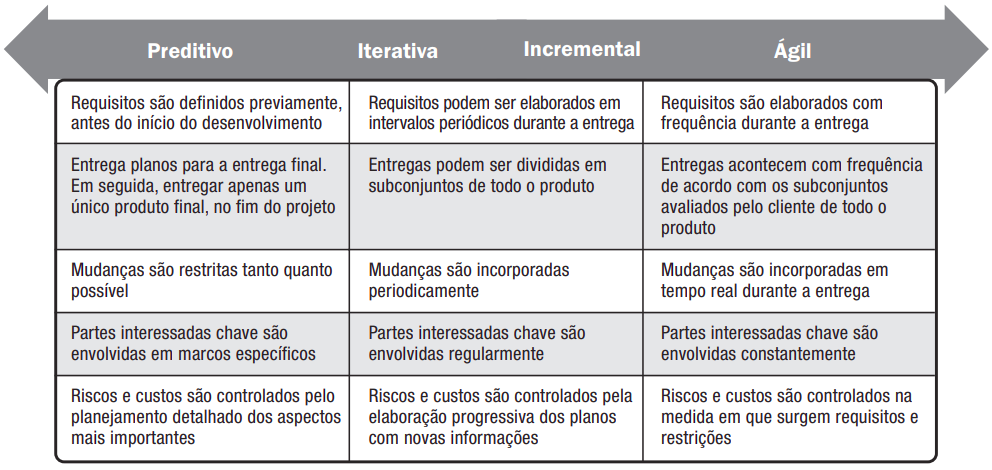
\includegraphics[width=\textwidth]{src/tex/img/PreditivoAgilPMBOKpg666.png}
    \label{PreditivoAgilPMBOK}
    \textbf{Fonte:} PMBOK \cite{PMBOK:2017}
\end{figure}


\subsection{Lean}
\subsection{XP}
\subsection{Scrum}
\subsection{Kanban}
\subsection{Scrumban}

\chapter{Estado da arte}
\label{sec:EstadoArte}


\chapter{Proposta do Trabalho}
\label{sec:Proposta}


\chapter{Experimentos e Discussão}
\label{sec:Experimentos}


\chapter{Conclusões e Trabalhos Futuros}
\label{sec:Conclusoes}


  \postextual


  % ----------------------------------------------------------
  % Referências bibliográficas
  % ----------------------------------------------------------
  \bibliography{references}
  
  % ----------------------------------------------------------
  % Glossário
  % ----------------------------------------------------------
  %
  % Consulte o manual da classe abntex2 para orientações sobre o glossário.
  %
  %\glossary

  % ----------------------------------------------------------
  % Apêndices
  % ----------------------------------------------------------

  % ---
  % Inicia os apêndices
  % ---
  \begin{apendicesenv}

  % Imprime uma página indicando o início dos apêndices
  \partapendices

  % ----------------------------------------------------------
  % \chapter{Nullam elementum urna vel imperdiet sodales elit ipsum pharetra ligula
  % ac pretium ante justo a nulla curabitur tristique arcu eu metus}
  % ----------------------------------------------------------
  % \lipsum[55-57]

  \end{apendicesenv}
  % ---


  % ----------------------------------------------------------
  % Anexos
  % ----------------------------------------------------------

  % ---
  % Inicia os anexos
  % ---
  % \begin{anexosenv}

  % Imprime uma página indicando o início dos anexos
  % \partanexos

  % ---
  % \chapter{Morbi ultrices rutrum lorem.}
  % ---
  % \lipsum[30]

  % ---
  % \chapter{Cras non urna sed feugiat cum sociis natoque penatibus et magnis dis
  % parturient montes nascetur ridiculus mus}
  % ---

  % \lipsum[31]

  % ---
  % \chapter{Fusce facilisis lacinia dui}
  % ---

  % \lipsum[32]

  % \end{anexosenv}

  %---------------------------------------------------------------------
  % INDICE REMISSIVO
  %---------------------------------------------------------------------

  \printindex

  \end{document}
